\documentclass{article}
\usepackage[a4paper, margin=1in]{geometry}
\usepackage[T1]{fontenc}
\usepackage[utf8]{inputenc}
\usepackage{amsmath, amssymb, graphicx, hyperref}
\usepackage{bookmark}
\graphicspath{{../figures/}}
\usepackage[framed,numbered]{matlab-prettifier}
\usepackage{xcolor}
\usepackage{listings}

\geometry{a4paper, margin=1in}

% MATLAB code style
\lstset{
  style      = Matlab-editor,
  basicstyle = \mlttfamily,
  breaklines = true
}

\title{\textbf{Practical - 7}}
\author{}
\date{October 22, 2026}

\pagenumbering{gobble}

\begin{document}
\maketitle

\noindent
\textbf{\large{Aim:}} To analyze a lake pollution model with constant and seasonal flow of pollutant concentration.

\vspace{1em}
\noindent
\textbf{\large{Theory:}} 

\noindent
The main idea is to model how the amount of pollutant in a lake changes with time.

\vspace{0.5em}
\noindent
\textbf{Basic Idea:} Suppose a lake contains water and some pollutants.

\noindent
There can be:
\begin{enumerate}
    \item Polluted water entering the lake.
    \item Water leaving the lake.
    \item Pollutant entering with the incoming water.
    \item pollutant leaving with the outgoing water.
\end{enumerate}

\noindent
The fundamental principle is:
\begin{center}
    Rate of change = Rate in - Rate out
\end{center}

\vspace{2em}
\noindent
\begin{center}
\textbf{\underline{Case I: Constant Flow}}
\end{center}

\noindent
Define the variables

\noindent
Suppose
\begin{enumerate}
    \item $V =$ volume of water in lake
    \item $r =$ inflow rate
    \item $c_{in} =$ pollutant concentration in incoming water
    \item $\frac{x}{V} =$ pollutant concentration inside the lake
\end{enumerate}

\noindent
Therefore,

\noindent
Pollutant entering 
\begin{center}
    Rate in = $rc_{in}$
\end{center}

\noindent
Pollutant leaving, since the concentration in the lake is $\frac{x}{V}$, the pollutant leaving is
\begin{center}
    Rate out = $r\frac{x}{V}$
\end{center}

\noindent
Therefore: 
\[\frac{dx}{dt} = rc_{in} - r\frac{x}{V}\]
This is the first-order linear ODE.

\vspace{2em}
\noindent
Example:

\noindent
Suppose:
\begin{center}
    $V =$ 1000 litres, \\
    $r =$ 100 litres/day
\end{center}
and pollutant concentration entering is 
\begin{center}
    $c_{in} =$ 0.01 kg/litre
\end{center}

\vspace{2em}
\noindent
Initially, suppose
\[x(0) = 20\]
Then
\[\frac{dx}{dt} = 100(0.01) - \frac{100}{1000}x\]
Therefore:
\begin{center}
    $\frac{dx}{dt} = 1 - 0.1x$ with \\
    $x(0) = 20$
\end{center}

\vspace{2em}
\noindent
\begin{center}
\textbf{\underline{Case II: Seasonal Flow}}
\end{center}

\noindent
Here, \[r = r(t)\]
\[r(t) = 100 + 20 \sin{t}\]
This represent a flow varies periodically around and average value of 100.

\noindent
Same as above model, we get
\[\frac{dx}{dt} = (1000+20\sin{\omega t})(0.01) - (\frac{100+20\sin{\omega t}}{1000}x)\]
\[x(0) = 20\]

\vspace{1em}
\noindent
\textbf{\large{MATLAB Code (Constant Flow):}}
\begin{lstlisting}
clc; clear all; close all;
            
syms x(t)
            
V= 1000; % flow rate
r=100; % incoming concentration
c_in = 0.01;
eqn = diff(x,1) == r*c_in - (r/V)*x; %% dx/dt = rate entering -rate leaving
init = x(0) == 20; %at t=0, the lake contains 20 units of pollutant.
xsol = dsolve(eqn, init);
disp(xsol)
fplot(xsol, [0,50])
grid on
title('Lake Pollution Model- Constant flow')
xlabel('Time')
ylabel('Amount of pollutant')
\end{lstlisting}

\newpage
\noindent
\textbf{\large{Output (Constant Flow):}}
\begin{flushleft}
$10\,{\mathrm{e}}^{-\frac{t}{10}} +10$
\end{flushleft}
\begin{figure}[htbp]
    \centering
    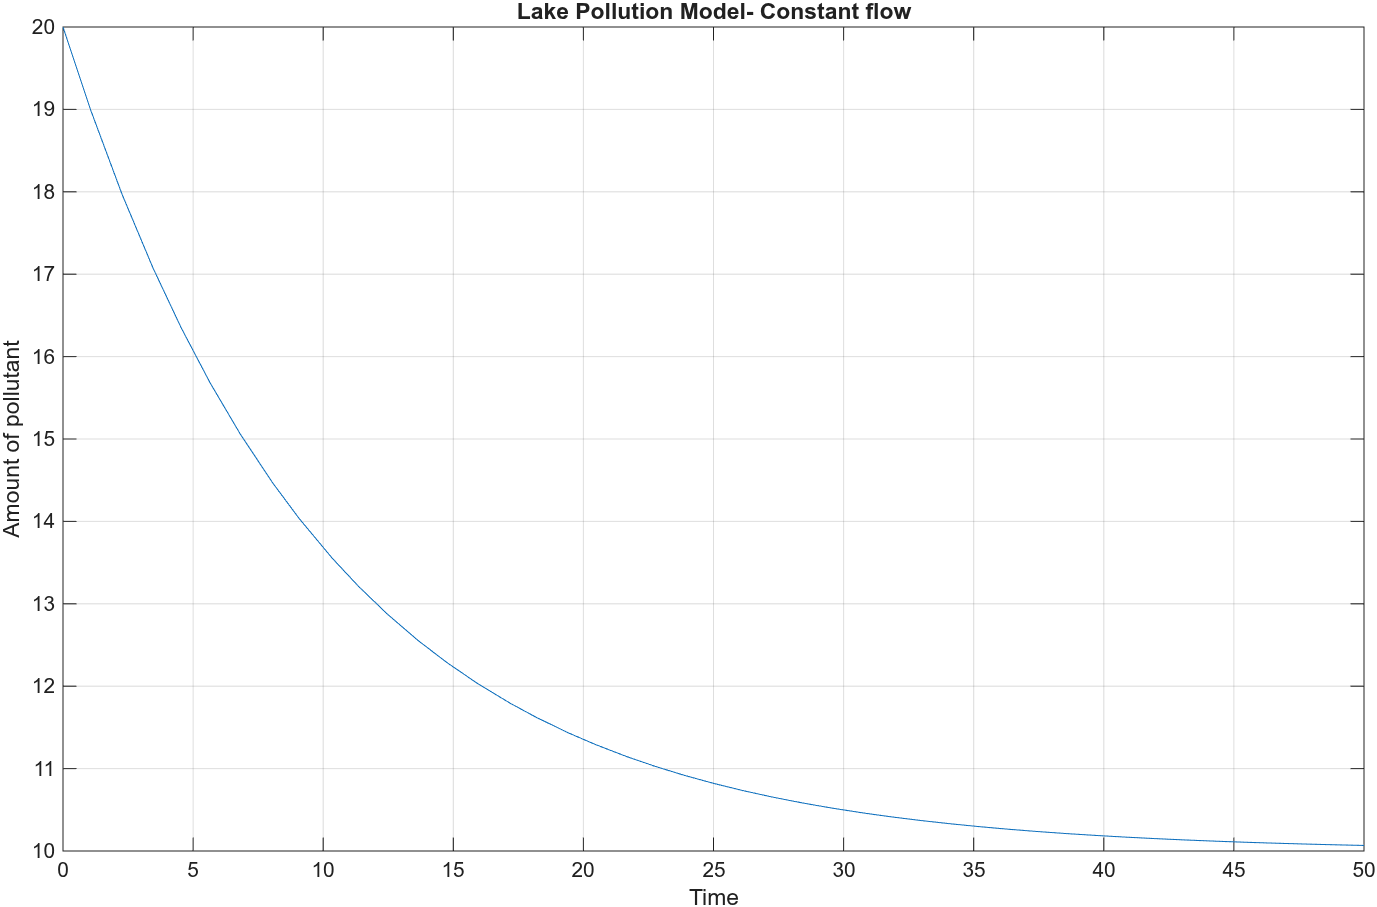
\includegraphics[width=0.7\textwidth]{Figure7.1.png}
\end{figure}

\vspace{1em}
\noindent
\textbf{\large{MATLAB Code (Seasonal Flow):}}
\begin{lstlisting}
clc; clear all; close all;
            
syms x(t)
            
V= 1000; % flow rate
r=100; % incoming concentration
c_in = 0.01;
eqn = diff(x,1) == r*c_in - (r/V)*x; %% dx/dt = rate entering -rate leaving
init = x(0) == 20; %at t=0, the lake contains 20 units of pollutant.
xsol = dsolve(eqn, init);
disp(xsol)
fplot(xsol, [0,50])
grid on
title('Lake Pollution Model- Seasonal flow')
xlabel('Time')
ylabel('Amount of pollutant')
\end{lstlisting}

\vspace{1em}
\noindent
\textbf{\large{Output (Seasonal Flow):}}
\begin{flushleft}
$10000-9980\,{\mathrm{e}}^{\frac{73\,\cos \left(\frac{2\,\pi \,t}{365}\right)}{40\,\pi }-\frac{t}{1000}} \,{\mathrm{e}}^{-\frac{73}{40\,\pi }}$
\end{flushleft}

\newpage
\begin{figure}[htbp]
    \centering
    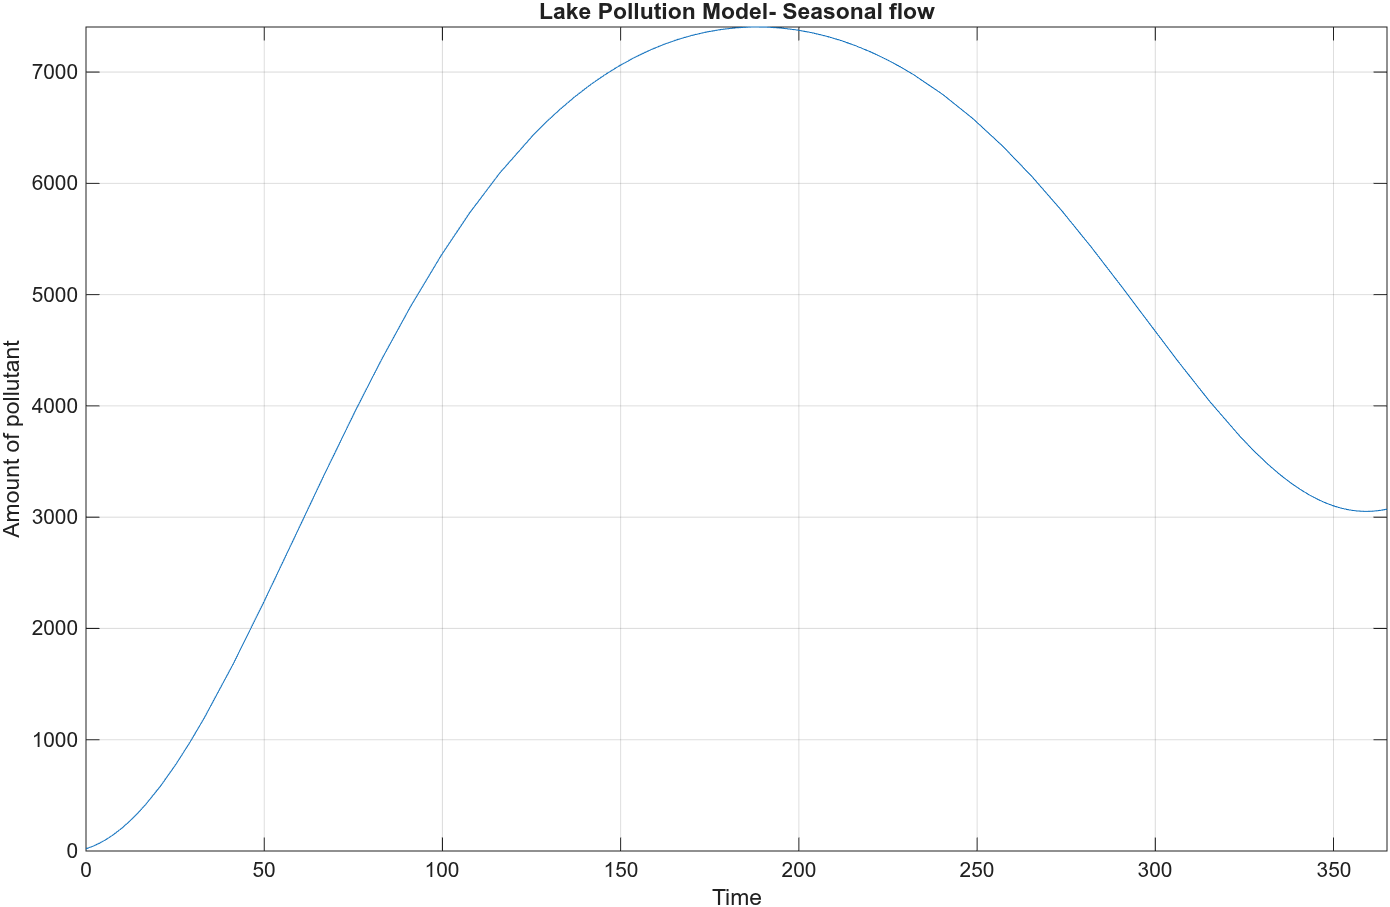
\includegraphics[width=0.7\textwidth]{Figure7.2.png}
\end{figure}

\end{document}
